% \subsection{Results}


\begin{figure}[tb]
    \begin{minipage}[h]{0.27\linewidth}
    \center{
        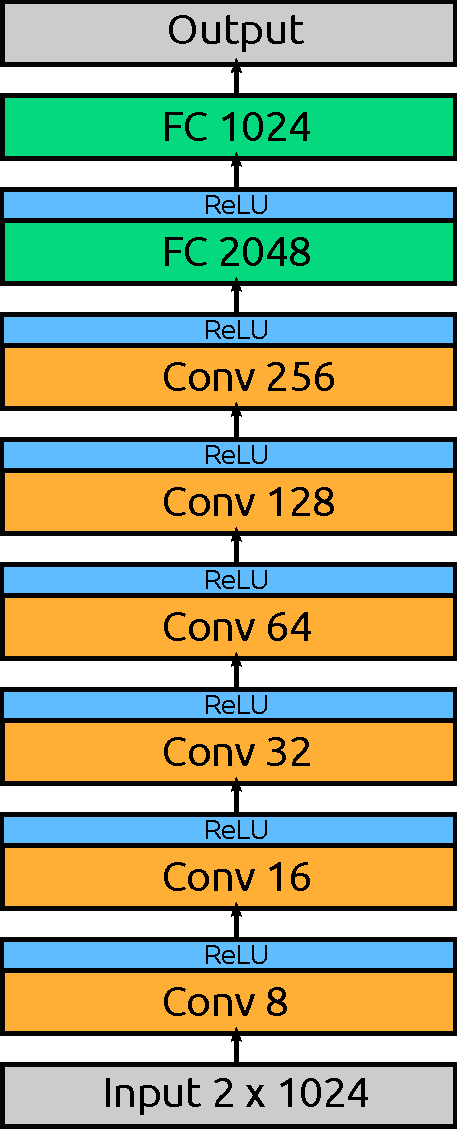
\includegraphics[width=1\linewidth]{images/nn_nft_inft/architecture_1.pdf} (a)
    }
    \end{minipage}
    \hfill
    \begin{minipage}[h]{0.72\linewidth}
        \begin{minipage}[h]{1.0\linewidth}
        \center{
            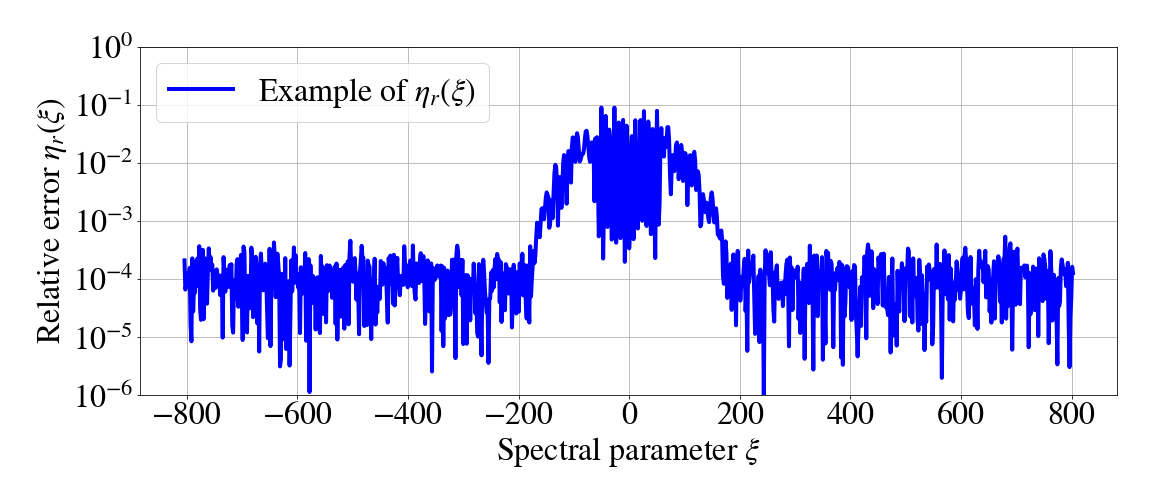
\includegraphics[width=1\linewidth]{images/nn_nft_inft/spectrum_rel_error_example_globecom.png} (b) \\
        }
        \end{minipage}
        \vfill
        \begin{minipage}[h]{1.0\linewidth}
        \center{
            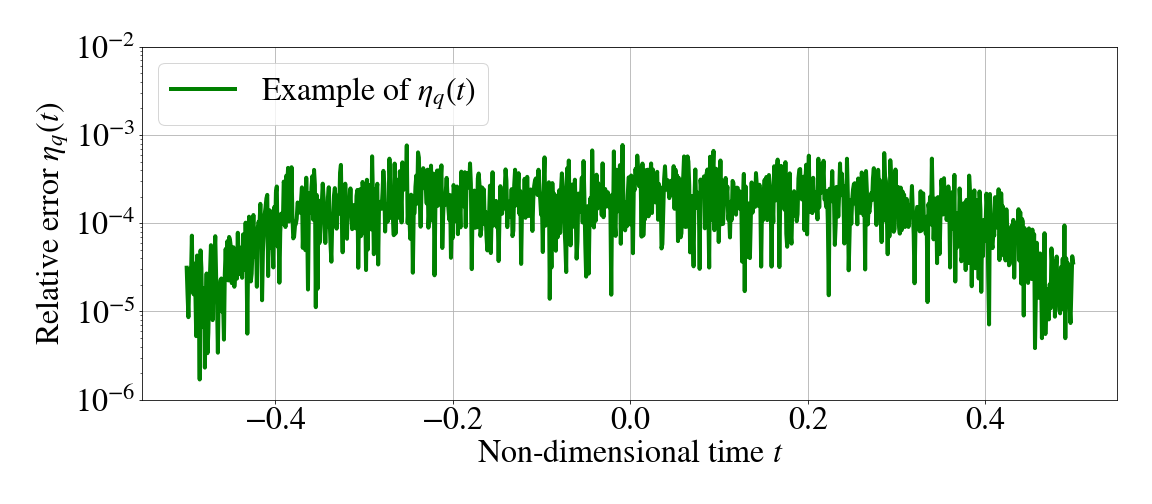
\includegraphics[width=1\linewidth]{images/nn_nft_inft/signal_rel_error_example_globecom.png} (c)
        }
        \end{minipage}
    \end{minipage}
    \caption{\textbf{(a)} Proposed architecture of the NN that performs the NFT operations. \textbf{(b)} Value of the relative error $\eta_r(\xi)$ between the precomputed and predicted continuous spectrum. \textbf{(c)} Value of the relative error $\eta_q(t)$ between the original and predicted signal.}
    \label{fig:arch_and_result_nn_nft}
\end{figure}

In this section, we use the NN to predict the continuous NFT spectrum of complex optical signals and transform the spectrum back (the inverse NFT) into a signal. 
To assess the quality of the NN prediction, we use the following formula defining the relative error for the continuous NFT spectrum:
\begin{equation}
    \eta_r(\xi) = \frac{|r_\text{predicted}(\xi) - r_\text{actual}(\xi)| }{\langle |r_\text{actual}(\xi)| \rangle_{\xi}} {,}
\end{equation}
where $\langle \cdot \rangle_{\xi}$ denotes the mean over the spectral interval, the ``predicted'' and ``actual'' indices refer to the NN-predicted and precomputed values of the reflection coefficient $r(\xi)$, respectively. A similar formula for calculating the relative error for signal prediction:
\begin{equation}
    \eta_q(t) = \frac{|q_\text{predicted}(t) - q_\text{actual}(t)| }{\langle |q_\text{actual}(t)| \rangle_{t}} {,}
\end{equation}
where $q(t)$ is a signal and $\langle \cdot \rangle_{t}$ here is the mean over the time interval. The above relative error $\eta_r(\xi)$ and $\eta_q(t)$ is determined at the point $\xi$ and $t$, respectively. We use $\langle \eta_r(\xi) \rangle_{\xi}$ and $\langle \eta_q(t) \rangle_{t}$ to estimate the overall mean of the error. We stress that the metric was chosen in such a way as to take into account even the regions where the value of the spectrum or signal is much less than one.

% \begin{figure}[tbp]
% \centerline{
%     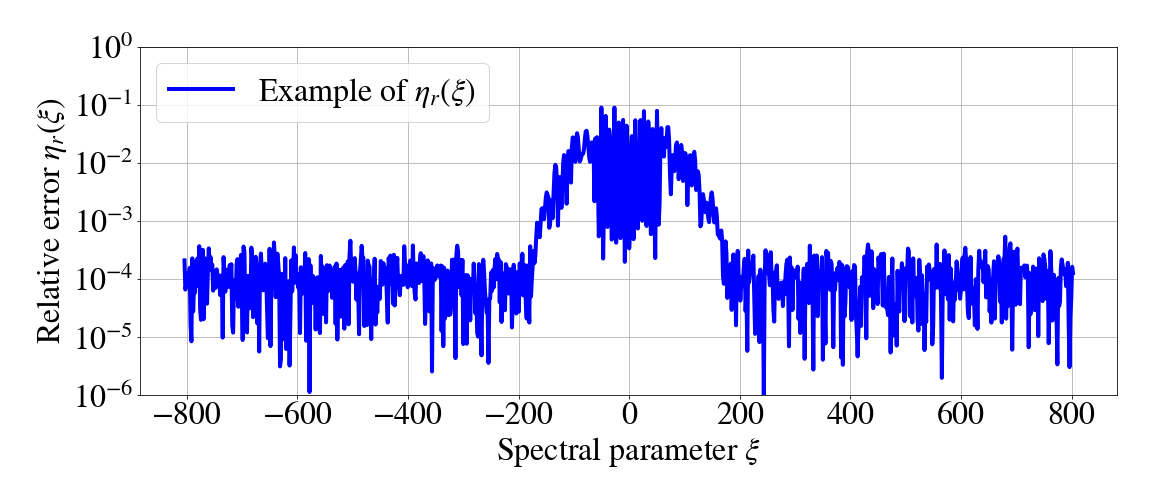
\includegraphics[width=1\linewidth]{images/nn_nft_inft/spectrum_rel_error_example_globecom.png}
% }
% \caption{Value of the relative error $\eta_r(\xi)$ between the precomputed and predicted continuous spectrum.}
% \label{fig:result_direct}
% \end{figure}

% \begin{figure}[tbp]
% \centerline{
%     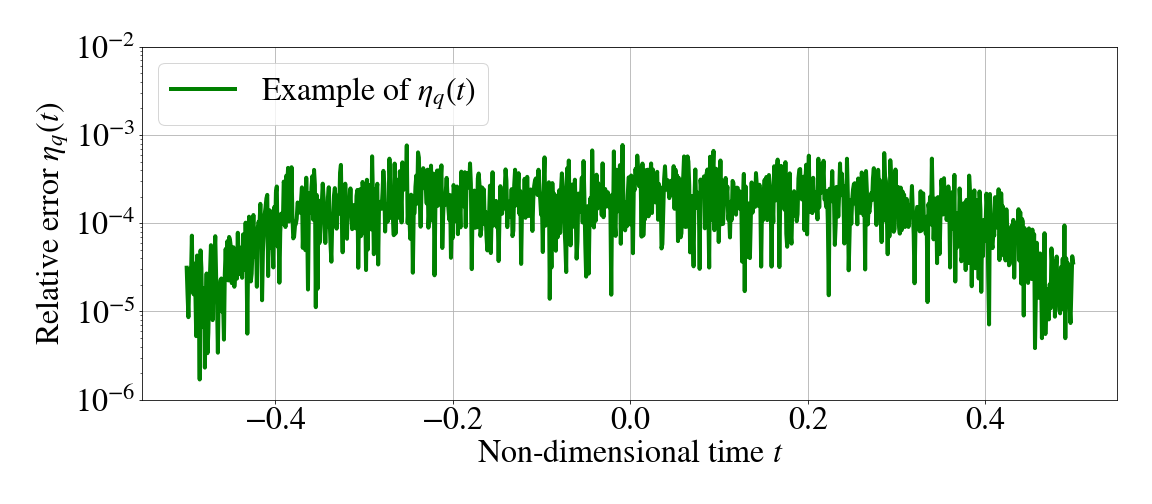
\includegraphics[width=1\linewidth]{images/nn_nft_inft/signal_rel_error_example_globecom.png}
% }
% \caption{Value of the relative error $\eta_q(t)$ between the original and predicted signal.}
% \label{fig:result_inverse}
% \end{figure}




Fig.~\ref{fig:arch_and_result_nn_nft}a shows the architecture of the NN that performs the NFT operations (direct and inverse transform), with the parameters given inside the figure. The NN consists of sequential convolution layers and fully connected output layers. At the input, the network receives a complex signal consisting of 1024 points. This NN predicts only one component of the continuous NF spectrum, such that two identical NNs have to be used to predict the real and imaginary $r(\xi)$ parts. Similarly, converting the spectrum back to a signal requires two separate NNs for the real and imaginary parts of the signal $q(t)$. Each of the four NNs with the same architectures we trained independently.

There are 94035 signals in the dataset, 9403 are used for validation and are not involved in the training process. To generate the signals, we used random data sequences encoded in the Quadrature Phase Shift Keying (QPSK) format. The energy of all signals is the same and is chosen at such a level that nonlinear effects are strong. At the selected energy, some of the signals contained a discrete spectrum, but such signals did not get into the training dataset. The continuous spectrum for each signal had been precomputed using the conventional direct NFT methods. To train the NN, we used the mean squared error (MSE) as the loss function. In training the NN, we employed the Adam (Adaptive Moment Estimation) optimisation algorithm with a learning rate of 1e-4. On average, with the amount of data used, our learning process took 50 000 epochs.

Fig.~\ref{fig:arch_and_result_nn_nft}b depicts $\eta_r(\xi)$ -- the difference between the predicted and actual (precomputed using conventional NFT method) continuous nonlinear spectrum for the example signal, while Fig.~\ref{fig:arch_and_result_nn_nft}c shows the example of $\eta_q(t)$ for the inverse NFT. We see from the graphs that NN performs both forward and inverse transformations with high accuracy. Some increase in the error at the centre for a continuous spectrum is associated with its localization in the middle. While at the edges of the spectral interval, $r(\xi)$ values tend to $0$. There is no such feature for the signal since it is evenly located over the entire time interval.
The mean value over the entire validation set of the mean relative prediction error of the continuous spectrum $\langle \eta_r(\xi) \rangle_{\xi}$ for NN forward NFT is $2.68 \cdot 10^{-3}$. For the inverse transformation, the mean over the entire validation set of the mean relative signal prediction error $\langle \eta_q(t) \rangle_{t} = 1.62 \cdot 10^{-4}$.
The results obtained show that the presented architecture can perform forward and backward NFT with high accuracy.


%-------------------------------------------------- Conclusions Section ———————————————————————————%

% \subsection{Conclusions}

% At the moment, ML and NN are state-of-the-art technologies that are actively researched in the fields of nonlinear signal processing and optical communications.
% The proposed NN architecture demonstrates the fundamental possibility of using the NNs to analyze and (de)modulate the complex optical signals used in communications. This opens up the prospects for improving existing systems without the need for a deep understanding of the internal nonlinear processes that affect the quality of signal transmission.
% We would like to stress that the method proposed in our current work is only the first step in the development of methods for machine processing of optical signals. It can be used to create smart receivers with digital back-propagation algorithms based on NFT and NN.
% Our findings demonstrate that the use of NN can allow studying not only the internal structure but also generating new signals using autoencoders. The fundamental possibility of using NN for NFT, in fact, can set up new areas for research related to the analysis of inherently nonlinear signal's structure and evolution characteristics. The next step in this direction can be the generalization of the results obtained in our work for the sake of our addressing the case of symbol sequences and simulating signal propagation in the NLSE-type channels.